\documentclass[12pt]{extarticle}
\usepackage[left = 2cm, right = 2cm, top = 2cm, bottom = 2cm]{geometry}
\usepackage{graphicx}
\usepackage{amsmath}
\usepackage{amssymb}
\usepackage{hyperref}
\usepackage{listings}
\usepackage{multirow}

\begin{document}

\begin{flushleft}
\begin{LARGE}
\textbf{16.5}
\end{LARGE}  
\end{flushleft}

\vfill
\begin{center}
\begin{Huge}Permutation Groups\end{Huge}
\end{center}
\vfill

\pagebreak

\begin{center}
\textbf{Question 1}
\end{center}

We will identify permutations with arrays in the following way: the array $(a_1,a_2,\dots, a_n)$ represents the permutation $1 \rightarrow a_1, \, 2 \rightarrow a_2$ and so on. Here are some outputs from the inverse and product programs.
$$(2,3,6,5,1,4)^{-1} =  (5,1,2,6,4,3)$$
$$(2,3,6,5,1,4)\cdot (4,3,5,1,2,6) = (5,6,1,2,3,4)$$

So both programmes work as expected. The complexity of the inverse procedure is $O(n^2)$: for each $k \in [n]$   
it iterates through, on average, half the positions of the array, of which there are $n/2$.\\

We will henceforth denote the set of permutations $\{ \pi_1, \dots ,\pi_k \}$  by the $n \times k$ array 

$$\begin{pmatrix} 
  \uparrow &  &  \uparrow \\ 
  \pi_1 & \dots &  \pi_k \\ 
  \downarrow &  &  \downarrow \\ 
\end{pmatrix} $$

We will also make use of the standard notation throughout.


\begin{center}
\textbf{Question 2}
\end{center}

For each $1 \leq i \leq n$ let $\pi_i$ and $\pi_i'$ denote the original and modified permutations respectively. \\

\textbf{Modified set generates the group.} If $\pi_i'$ is in the array then we know that $\pi_i' = g^{-1}\pi_i$ for some $g$ expressible as a product of $\pi_j'$ permutations for $j<i$ in the array. So $\pi_i = g\pi_i'$ and we can generate all the $\pi_i$ from permutations only in the array.

If $\pi_i'$ is not in the array (it is the identity) then we know that $g^{-1}\pi_i = e$ for some $g$ expressible as a product of $\pi_j'$  permutations for $j<i$ in the array. So $\pi_i = g$ and we can generate all the $\pi_i$ again. 

Hence the modified set of permutations generates the same group.\\

\textbf{Size of modified set.} If a permutation is put in position $(i,j)$ in the array then it must fix all $a<i$ and send $i$ to $j$. Hence $j>i$ since the permutation is bijective (and hence injective) and it does not fix $i$. So we can only place permutations in the top triangle, giving at most $n(n-1)/2$ generators. The size of the modified set of generators is also at most the size of the original set. So it is at most $\min (k,n(n-1)/2)$.\\

\textbf{Complexity.} The loop iterating through the elements of the generating set contributes a factor of $O(k)$. The loop iterating through $[n]$ contributes a factor of $O(n)$. Inside the loop the storing of permutations in the array $A$ contributes another factor of $O(n)$. So the overall complexity is $O(kn^2)$.

\begin{center}
\textbf{Question 3}
\end{center}

We will give a few examples to show the program is working correctly.\\

\textbf{Example 1.} The following set contains all elements of the group $S_3$. 

$$\begin{pmatrix} 
  1 &  1 &  2 &  2 &  3 &  3 \\ 
  2 &  3 &  1 &  3 &  1 &  2 \\ 
  3 &  2 &  3 &  1 &  2 &  1 \\ 
\end{pmatrix} $$


From the Stripping Algorithm of Sims we obtain the array $A$ and hence the reduced set of permutations. In the procedure the array $A$ from the question has been modified to a $n^2 \times n$ array so that the permutations may be written out in full. 

$$\begin{pmatrix} 
  0 &  2 &  3 \\ 
  0 &  1 &  1 \\ 
  0 &  3 &  2 \\ 
  0 &  0 &  1 \\ 
  0 &  0 &  3 \\ 
  0 &  0 &  2 \\ 
  0 &  0 &  0 \\ 
  0 &  0 &  0 \\ 
  0 &  0 &  0 \\ 
\end{pmatrix}
\longrightarrow
\begin{pmatrix} 
  1 &  2 &  3 \\ 
  3 &  1 &  1 \\ 
  2 &  3 &  2 \\ 
\end{pmatrix} $$

\textbf{Example 2.} The following set contains all the elements of the group $A_4$. 

$$\left(\begin{array}{*{12}c}
1 &  1 &  1 &  2 &  2 &  2 &  3 &  3 &  3 &  4 &  4 &  4 \\ 
  2 &  3 &  4 &  1 &  3 &  4 &  1 &  2 &  4 &  3 &  1 &  2 \\ 
  3 &  4 &  2 &  4 &  1 &  3 &  2 &  4 &  1 &  2 &  3 &  1 \\ 
  4 &  2 &  3 &  3 &  4 &  1 &  4 &  1 &  2 &  1 &  2 &  3 \\ 
\end{array}\right)$$

Using the program we have

$$\begin{pmatrix} 
  0 &  2 &  3 &  4 \\ 
  0 &  1 &  1 &  3 \\ 
  0 &  4 &  2 &  2 \\ 
  0 &  3 &  4 &  1 \\ 
  0 &  0 &  1 &  1 \\ 
  0 &  0 &  3 &  4 \\ 
  0 &  0 &  4 &  2 \\ 
  0 &  0 &  2 &  3 \\ 
  0 &  0 &  0 &  0 \\ 
  0 &  0 &  0 &  0 \\ 
  0 &  0 &  0 &  0 \\ 
  0 &  0 &  0 &  0 \\ 
  0 &  0 &  0 &  0 \\ 
  0 &  0 &  0 &  0 \\ 
  0 &  0 &  0 &  0 \\ 
  0 &  0 &  0 &  0 \\ 
\end{pmatrix} 
\longrightarrow
\begin{pmatrix} 
  1 &  1 &  2 &  3 &  4 \\ 
  3 &  4 &  1 &  1 &  3 \\ 
  4 &  2 &  4 &  2 &  2 \\ 
  2 &  3 &  3 &  4 &  1 \\ 
\end{pmatrix} $$

\begin{center}
\textbf{Question 4}
\end{center}

There is a bijection between the set of left cosets of $G_\alpha$ in $G$ and the orbit of $\alpha$, given by $\Psi: G/G_\alpha \to G \cdot \alpha,$ $ gG_\alpha \mapsto g\alpha$. Intuitively this is because the difference of two elements in the same coset is in the stabilizer and so they have the same effect on $\alpha$.

The orbit-stabilizer theorem states that for a finite group $G$ and an element $\alpha \in X$,  

$$|G| = |G \cdot \alpha||G_\alpha|$$

\begin{center}
\textbf{Question 5}
\end{center}

\textbf{Description.} First apply every permutation in the generating set to $\alpha$ and add every new orbit element to the list. Continue by repeating this with every element in the list. Stop once no new elements are found. Keeping track of the permutations used allows each witness to be computed.\\

\textbf{Explanation.} For every element $\beta \in X$ in the orbit of $\alpha$ there is some $g \in G$ with $g\alpha = \beta$. If $g$ is in the generating set then $\beta$ will be added after the first iteration. Otherwise $g$ can be written as a product of $m$ elements from the generating set. By induction on $m$ at some point $\beta$ will be added to the list, since both the group $G$ and the set $X$ are finite.\\

  

We will give a few examples to show the program works as required.\\

\textbf{Example 1}. Take the subgroup of $S_5$ generated by the permutations $(123)$ and $(45)$.

$$\begin{pmatrix} 
  2 &  1 \\ 
  3 &  2 \\ 
  1 &  3 \\ 
  4 &  5 \\ 
  5 &  4 \\ 
\end{pmatrix} $$

The elements of the orbits are displayed in the top row of the matrices in bold with a witness below each one. The results are shown for the elements $2$ and $4$.

$$\begin{pmatrix} 
  \textbf{2} &  \textbf{3} &  \textbf{1} \\ 
  1 &  2 &  3 \\ 
  2 &  3 &  1 \\ 
  3 &  1 &  2 \\ 
  4 &  4 &  4 \\ 
  5 &  5 &  5 \\ 
\end{pmatrix} 
,
\begin{pmatrix} 
  \textbf{4} &  \textbf{5} \\ 
  1 &  1 \\ 
  2 &  2 \\ 
  3 &  3 \\ 
  4 &  5 \\ 
  5 &  4 \\ 
\end{pmatrix} $$

\textbf{Example 2}. Take the subgroup of $S_6$ generated by the permutations $(14)$, $(36)$ and $(24)$.

$$\begin{pmatrix} 
  4 &  1 &  1 \\ 
  2 &  2 &  4 \\ 
  3 &  6 &  3 \\ 
  1 &  4 &  2 \\ 
  5 &  5 &  5 \\ 
  6 &  3 &  6 \\ 
\end{pmatrix} $$

The results are shown for the elements $2$, $5$ and $6$.

$$\begin{pmatrix} 
  \textbf{2} &  \textbf{4} &  \textbf{1} \\ 
  1 &  1 &  4 \\ 
  2 &  4 &  1 \\ 
  3 &  3 &  3 \\ 
  4 &  2 &  2 \\ 
  5 &  5 &  5 \\ 
  6 &  6 &  6 \\ 
\end{pmatrix} 
,
\begin{pmatrix} 
  \textbf{5} \\ 
  1 \\ 
  2 \\ 
  3 \\ 
  4 \\ 
  5 \\ 
  6 \\ 
\end{pmatrix}
,
\begin{pmatrix} 
  \textbf{6} &  \textbf{3} \\ 
  1 &  1 \\ 
  2 &  2 \\ 
  3 &  6 \\ 
  4 &  4 \\ 
  5 &  5 \\ 
  6 &  3 \\ 
\end{pmatrix} $$

So indeed the program works as expected.\\

\begin{center}
\textbf{Question 6}
\end{center}

We consider the action of $t_{i+1}$ on $\alpha$

$$t_{i+1}\alpha = \varphi(y_it_i)\alpha = y_it_i\alpha$$

Using the definition of $\varphi$.

$$t_{r+1}\alpha = y_rt_r\alpha = y_r\dots y_1 t_1 \alpha = xt_1\alpha = x\alpha = \alpha$$

Since both $x$ and $t_1$ are in $G_\alpha$. So $t_{r+1}$ is also in $G_\alpha$. Since it is also in $T$ so we must have $t_{r+1} = t_1$.\\

We now show that $G_\alpha = \langle\lbrace \varphi(yt)^{-1}\cdot y\cdot t|y \in Y, t \in T \rbrace \rangle$.

$$yt\alpha = \varphi(yt)\alpha \Rightarrow \varphi(yt)^{-1}yt\alpha = \alpha \Rightarrow \varphi(yt)^{-1}yt \in G_\alpha$$

$\forall y \in Y, t \in T $. So $\langle \lbrace \varphi(yt)^{-1}\cdot y\cdot t|y \in Y, t \in T \rbrace \rangle \subseteq G_\alpha$.\\

Now $\forall x \in G_\alpha$, write $x = y_r\dots y_1$ with each $y_i$ an element of $Y$. Choose $t_1 = e$ and construct the other $t_i$ recursively by $t_{i+1} = \varphi(y_it_i)$.

$$x = y_r\dots y_1 = (t_{r+1}^{-1}y_rt_r)(t_r^{-1}y_{r-1}t_{r-1})\dots (t_2^{-1}y_1t_1)$$
$$ = [\varphi(y_rt_r)^{-1}y_rt_r][\varphi(y_{r-1}t_{r-1})^{-1}y_{r-1}t_{r-1}]\dots  [\varphi(y_1t_1)^{-1}y_1t_1]$$

Using $t_{r+1} = t_1 = e$. This is a product of elements from the set. Hence $ G_\alpha \subseteq \langle \lbrace \varphi(yt)^{-1}\cdot y\cdot t|y \in Y, t \in T \rbrace \rangle$ and so the two are in fact equal.

\begin{center}
\textbf{Question 7}
\end{center}

This program iterates through all elements in both sets $T$ and $Y$ and uses the result from question 6 to find a generating set for the stabilizer. We will use the same examples used in Question 5 to show the program works as required.\\

\textbf{Example 1}. The procedure yields the following generating sets for the stabilizers of the elements $2$ and $4$.

$$\begin{pmatrix} 
  1 \\ 
  2 \\ 
  3 \\ 
  5 \\ 
  4 \\ 
\end{pmatrix} 
,
\begin{pmatrix} 
  2 \\ 
  3 \\ 
  1 \\ 
  4 \\ 
  5 \\ 
\end{pmatrix} $$

\textbf{Example 2}. The procedure yields the following generating sets for the stabilizers of the elements $2$, $5$ and $6$.

$$\begin{pmatrix} 
  1 &  4 \\ 
  2 &  2 \\ 
  6 &  3 \\ 
  4 &  1 \\ 
  5 &  5 \\ 
  3 &  6 \\ 
\end{pmatrix} 
,
\begin{pmatrix} 
  2 &  1 &  1 \\ 
  1 &  2 &  4 \\ 
  3 &  6 &  3 \\ 
  4 &  4 &  2 \\ 
  5 &  5 &  5 \\ 
  6 &  3 &  6 \\ 
\end{pmatrix} 
,
\begin{pmatrix} 
  2 &  1 \\ 
  1 &  4 \\ 
  3 &  3 \\ 
  4 &  2 \\ 
  5 &  5 \\ 
  6 &  6 \\ 
\end{pmatrix} $$

\textbf{Complexity.} In the worst case, the set of witnesses $T$ contains $n$ elements (when the action is transitive). There are at most $k$ elements in the set of generators $Y$. Inside the loops, the inverse function dominates (since multiplication is linear in $n$) and therefore there is a contribution of $O(n^2)$. Hence the overall complexity of the algorithm is $O(kn^3)$. \\

To test this, the procedure was timed for a few different values of $n$ (the value of $k$ used was 5 and the permutations were randomised). The results are recorded below. The gradient of the plot is about 2.5 which suggests that the calculation above is indeed correct. 

\begin{table}[!htbp]
\centering
\begin{tabular}{|c|cccccccccc|}
\hline
\multirow{1}{2.5em}{$n$} & 80 &100 &120 &140 &160 &180 &200 &220 &240 &260 \\
\hline
\multirow{1}{2.5em}{Time} & 4.581 &7.489 &10.394 &14.483 &20.245 &25.948 &35.4 &42.793 &52.017 &71.029\\
\hline
\end{tabular}
\caption{Running times of stabilizer procedure}
\label{Table:1}
\end{table}

\begin{figure}[!htbp]
\centering
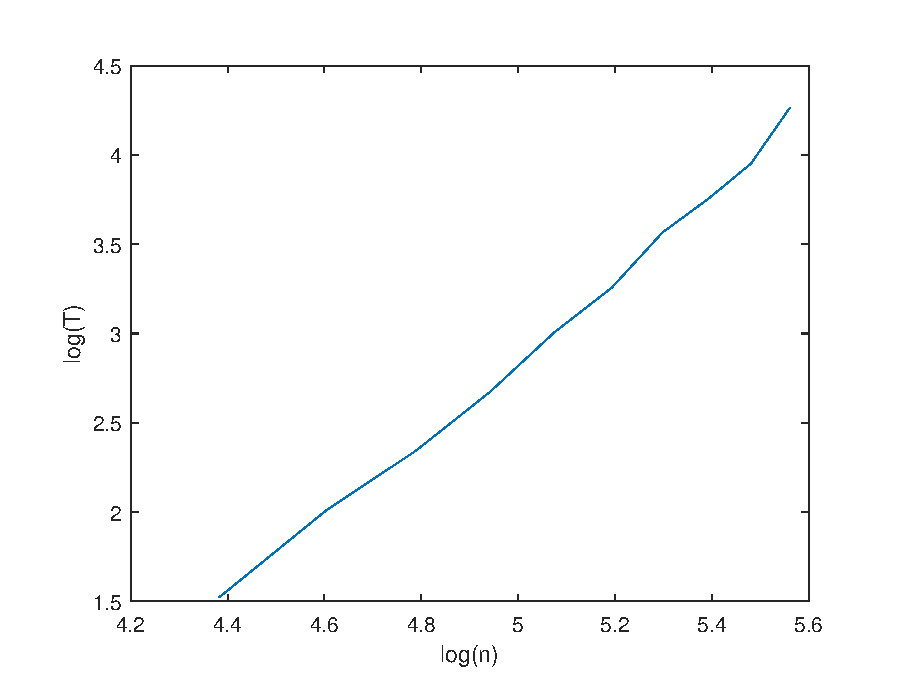
\includegraphics[scale=0.69]{Complexity.eps}\\
\caption{plot of log(T) against log(n)}
\label{figure:1}
\end{figure}
\pagebreak
\begin{center}
\textbf{Question 8}
\end{center}

\textbf{Procedure.} We construct the following chain of subgroups:

$$G\geq G_1 \geq G_{(1,2)} \dots \geq G_{(1,\dots,n)} = e$$

From which we obtain

$$|G| = |\mathcal{O}_G(1)||G_1| = |\mathcal{O}_G(1)||\mathcal{O}_{G_1}(2)||G_{(1,2)}| = \dots = |\mathcal{O}_G(1)|\dots|\mathcal{O}_{G_{(1,\dots,n-1)}}(n)|$$

Where $G_{(1,\dots,k)}$ is the subgroup which fixes elements $1,\dots,k$ and $\mathcal{O}$ is the Orbit. So by finding the subgroups iteratively and the sizes of the orbits, the order of the group can be determined.\\

\textbf{Example.} The following permutations generate $S_5$

$$\begin{pmatrix} 
  2 &  1 \\ 
  1 &  3 \\ 
  3 &  4 \\ 
  4 &  5 \\ 
  5 &  2 \\ 
\end{pmatrix} $$

Subgroup $G_1$ of order 24, before and after stripping.

$$\begin{pmatrix} 
  1 &  1 &  1 &  1 \\ 
  3 &  5 &  4 &  2 \\ 
  4 &  3 &  3 &  5 \\ 
  5 &  4 &  2 &  3 \\ 
  2 &  2 &  5 &  4 \\ 
\end{pmatrix}
\longrightarrow
\begin{pmatrix} 
  1 &  1 &  1 &  1 \\ 
  3 &  5 &  4 &  2 \\ 
  4 &  3 &  3 &  5 \\ 
  5 &  4 &  2 &  3 \\ 
  2 &  2 &  5 &  4 \\ 
\end{pmatrix} $$
     
Subgroup $G_{(1,2)}$ of order 6.

$$\begin{pmatrix} 
  1 &  1 &  1 \\ 
  2 &  2 &  2 \\ 
  5 &  3 &  4 \\ 
  3 &  5 &  5 \\ 
  4 &  4 &  3 \\ 
\end{pmatrix} 
\longrightarrow
\begin{pmatrix} 
  1 &  1 &  1 \\ 
  2 &  2 &  2 \\ 
  5 &  3 &  4 \\ 
  3 &  5 &  5 \\ 
  4 &  4 &  3 \\ 
\end{pmatrix} $$

Subgroup $G_{(1,2,3)}$ of order 2.

$$\begin{pmatrix} 
  1 \\ 
  2 \\ 
  3 \\ 
  5 \\ 
  4 \\ 
\end{pmatrix} 
\longrightarrow
\begin{pmatrix} 
  1 \\ 
  2 \\ 
  3 \\ 
  5 \\ 
  4 \\ 
\end{pmatrix} $$

The program outputs 120 for the order which is indeed correct. \\

\textbf{Need for Stripping Algorithm.} The procedure was executed with the permutations $(12)$ and $(12\dotsm 20)$, which generate $S_{20}$. It was performed twice and timed, once using the Stripping Algorithm at every stage (this took 573s) and once without using it (this ran over 4000s and was halted before completion). So we see that not using the Stripping Algorithm significantly increases the time required. 

\begin{center}
\textbf{Question 9}
\end{center}

We will show that $S_n$ is generated by the cycles $(12)$ and $(12\dotsm n)$. We know from 1A that for a permutation $\sigma \in S_n$ and a cycle $(a_1 \dotsm a_m) \in S_n$

$$\sigma (a_1 \dotsm a_m)\sigma^{-1} = (\sigma(a_1)\dotsm \sigma(a_m))$$

So $(12\dotsm n)(12)(12\dotsm n)^{-1} = (23)$ and we can iterate to generate all the transpositions of the form $(j,j+1)$. We can then obtain all transpositions $(i,j)$ (wlog $j > i)$ by 

$$(i,j) = (j,j-1)(j-1,j-2)\dots (i+2,i+1)(i,i+1)(i+1,i+2)\dots (j-1,j)$$

We can write every element in $S_n$ as a product of transpositions and so we can generate every element. Therefore $P_n > 0$ since there is always at least one pair of permutations that generates $S_n$.\\

If $g$ and $h$ are both even permutations then all the permutations they generate are also even, and so they can not generate $S_n$. Half of all permutations are even ($|A_n| = |S_n|/2$) so there is a 1/4 probability that both $g$ and $h$ are even. So independently of $n$, $P_n \leq 3/4$.\\

Estimates for $P_n$ have been calculated by generating 100 random pairs of permutations for each value of $n$. The values agree with the upper bound found above and are in fact quite close to it. 

\begin{table}[!htbp]
\centering
\begin{tabular}{|c|cccccccccc|}
\hline
\multirow{1}{1.5em}{$n$} & 5 & 6 & 7 & 8 & 9 & 10 & 11 &12 &13 & 14\\
\hline
\multirow{1}{1.5em}{$P_n$} & 0.42 & 0.36 & 0.68 & 0.62 & 0.68 & 0.73 & 0.65 & 0.66& 0.72 & 0.72\\
\hline
\end{tabular}
\caption{Estimates of $P_n$}
\label{Table:2}
\end{table}

\vspace{40mm}

\begin{center}
\textbf{End of Project}
\end{center}

\pagebreak
\begin{center}
\textbf{Product Function}
\end{center}
\lstinputlisting[language=Matlab]{Mul.m}

\begin{center}
\textbf{Inverse Function}
\end{center}
\lstinputlisting[language=Matlab]{Inv.m}

\begin{center}
\textbf{Stripping Algorithm of Sims}
\end{center}
\lstinputlisting[language=Matlab]{Sims.m}

\begin{center}
\textbf{Orbit Algorithm}
\end{center}
\lstinputlisting[language=Matlab]{Orb.m}

\begin{center}
\textbf{Representative function $\varphi$}
\end{center}
\lstinputlisting[language=Matlab]{Phi.m}

\begin{center}
\textbf{Stabilizer Algorithm}
\end{center}
\lstinputlisting[language=Matlab]{Stab.m}

\begin{center}
\textbf{Order Algorithm}
\end{center}
\lstinputlisting[language=Matlab]{Ord.m}

\begin{center}
\textbf{Questions 3,5,7,8}
\end{center}
\lstinputlisting[language=Matlab]{Untitled7.m}

\begin{center}
\textbf{Question 9}
\end{center}
\lstinputlisting[language=Matlab]{Question9.m}

\end{document}